
\section{Проектирование интеллектуальной системы}
\label{sec:designing}

\subsection{Общая архитектура интеллектуальной системы}

Интеллектуальная система ассистирования построена по трёхуровневой клиент-серверной архитектуре. На первом уровне расположен клиентский модуль — модификация игрового клиента, отвечающая исключительно за сбор и передачу событий. Второй уровень представляет собой серверное ядро, которое принимает поток событий, управляет состоянием диалогового контекста и принимает решения о необходимости генерации реплики. Третий уровень образуют внешние когнитивные сервисы, к которым сервер обращается для получения текста на естественном языке.

Помимо основного потока обработки данных, серверное ядро обслуживает административную веб-панель — браузерный интерфейс для мониторинга событий и управления параметрами системы. Взаимодействие всех участников — игрового клиента, сервера, внешних сервисов и панели управления — происходит асинхронно, что обеспечивает отзывчивость системы даже при задержках в обработке запросов.

% --- ДИАГРАММА: Компонентная диаграмма UML верхнего уровня ---
% Показать: Minecraft Client (Mod) <-> FastAPI Server <-> LLM Services
%           Browser (Admin Panel) <-> FastAPI Server
% ---

\subsection{Архитектура интерфейсного слоя}

\textbf{Структура модулей и слоёв}

Серверная часть системы разделена на несколько функциональных модулей с чёткими границами ответственности. Модуль приёма событий отвечает за регистрацию поступающих от игрового клиента данных и их буферизацию для последующего анализа. Модуль настроек обеспечивает хранение и изменение рабочих параметров системы, влияющих на поведение ассистента. Центральный модуль формирования реакций реализует логику принятия решений: он анализирует накопленные события, взаимодействует с когнитивными сервисами и определяет, когда и с каким содержанием следует сгенерировать реплику. Отдельный адаптерный модуль инкапсулирует взаимодействие с внешними языковыми моделями, скрывая от остальных компонентов детали конкретного провайдера.

Конфигурация системы, в том числе выбор активной языковой модели и параметры её работы, хранится во внешнем файле и может быть изменена без перезапуска сервера.

\textbf{Взаимодействие с внутренними компонентами}

Модули сервера обмениваются данными через общий буфер событий, хранящийся в оперативной памяти. Модуль формирования реакций при каждом запросе обращается к буферу за последними событиями, формирует на их основе запрос к языковой модели и возвращает готовую реплику.

Все обращения к внешним языковым сервисам выполняются асинхронно, чтобы не блокировать обработку остальных входящих запросов. При недоступности языковой модели система автоматически переключается на резервную логику, основанную на наборе правил, что обеспечивает непрерывность работы ассистента.

\subsection{Модели пользователей и сценарии использования}

\textbf{Ролевые модели пользователей и внешних систем}

В системе выделены четыре роли участников взаимодействия. Игрок является основным потребителем обратной связи: он получает реплики ассистента через внутриигровой интерфейс и может инициировать диалог, отправляя сообщения в игровой чат. Прямого доступа к серверу у игрока нет — всё взаимодействие осуществляется через клиентский мод. Администратор управляет системой через веб-панель: просматривает поток событий, изучает историю ответов ассистента, корректирует параметры поведения и выбирает языковую модель. В однопользовательском сценарии обе роли, как правило, совпадают. Игровой клиент выступает в роли автономного источника данных: он передаёт события серверу и исполняет поступающие от него команды. Внешний языковой сервис является поставщиком когнитивных функций: получив контекстный запрос, он возвращает текст реплики.

\textbf{Сценарии использования}

Выделены три основных сценария взаимодействия с интерфейсом системы.

Сценарий 1: автоматическая контекстная реакция ассистента (рисунок \ref{fig:sequence1}). Игровой клиент периодически опрашивает сервер, запрашивая актуальную реплику. Сервер формирует описание текущей ситуации на основе последних накопленных событий и передаёт его языковой модели. Полученная реплика проверяется на предмет избыточной частоты: если ситуация с момента последнего ответа существенно не изменилась, возвращается прежний результат. В случае критического события, например гибели персонажа, ограничение частоты снимается и реплика генерируется незамедлительно. При недоступности языковой модели ответ формируется резервной системой правил.

Сценарий 2: диалоговое взаимодействие (рисунок \ref{fig:sequence2}). Игрок вводит сообщение в игровой чат. Клиентский мод перехватывает его и отправляет на сервер вместе с контекстом последних событий. Сервер передаёт сообщение языковой модели, которая формулирует ответ в соответствии с заданным ролевым образом ассистента. Ответ возвращается игроку и сохраняется в истории взаимодействий.

Сценарий 3: мониторинг и настройка (рисунок \ref{fig:sequence3}). Администратор открывает веб-панель в браузере. На странице мониторинга события от игрового клиента отображаются в режиме реального времени по мере их поступления. На странице истории ответов доступна лента реплик ассистента. На странице настроек администратор изменяет параметры поведения системы и при необходимости переключает активную языковую модель.

\begin{figure}[H]
    \centering
    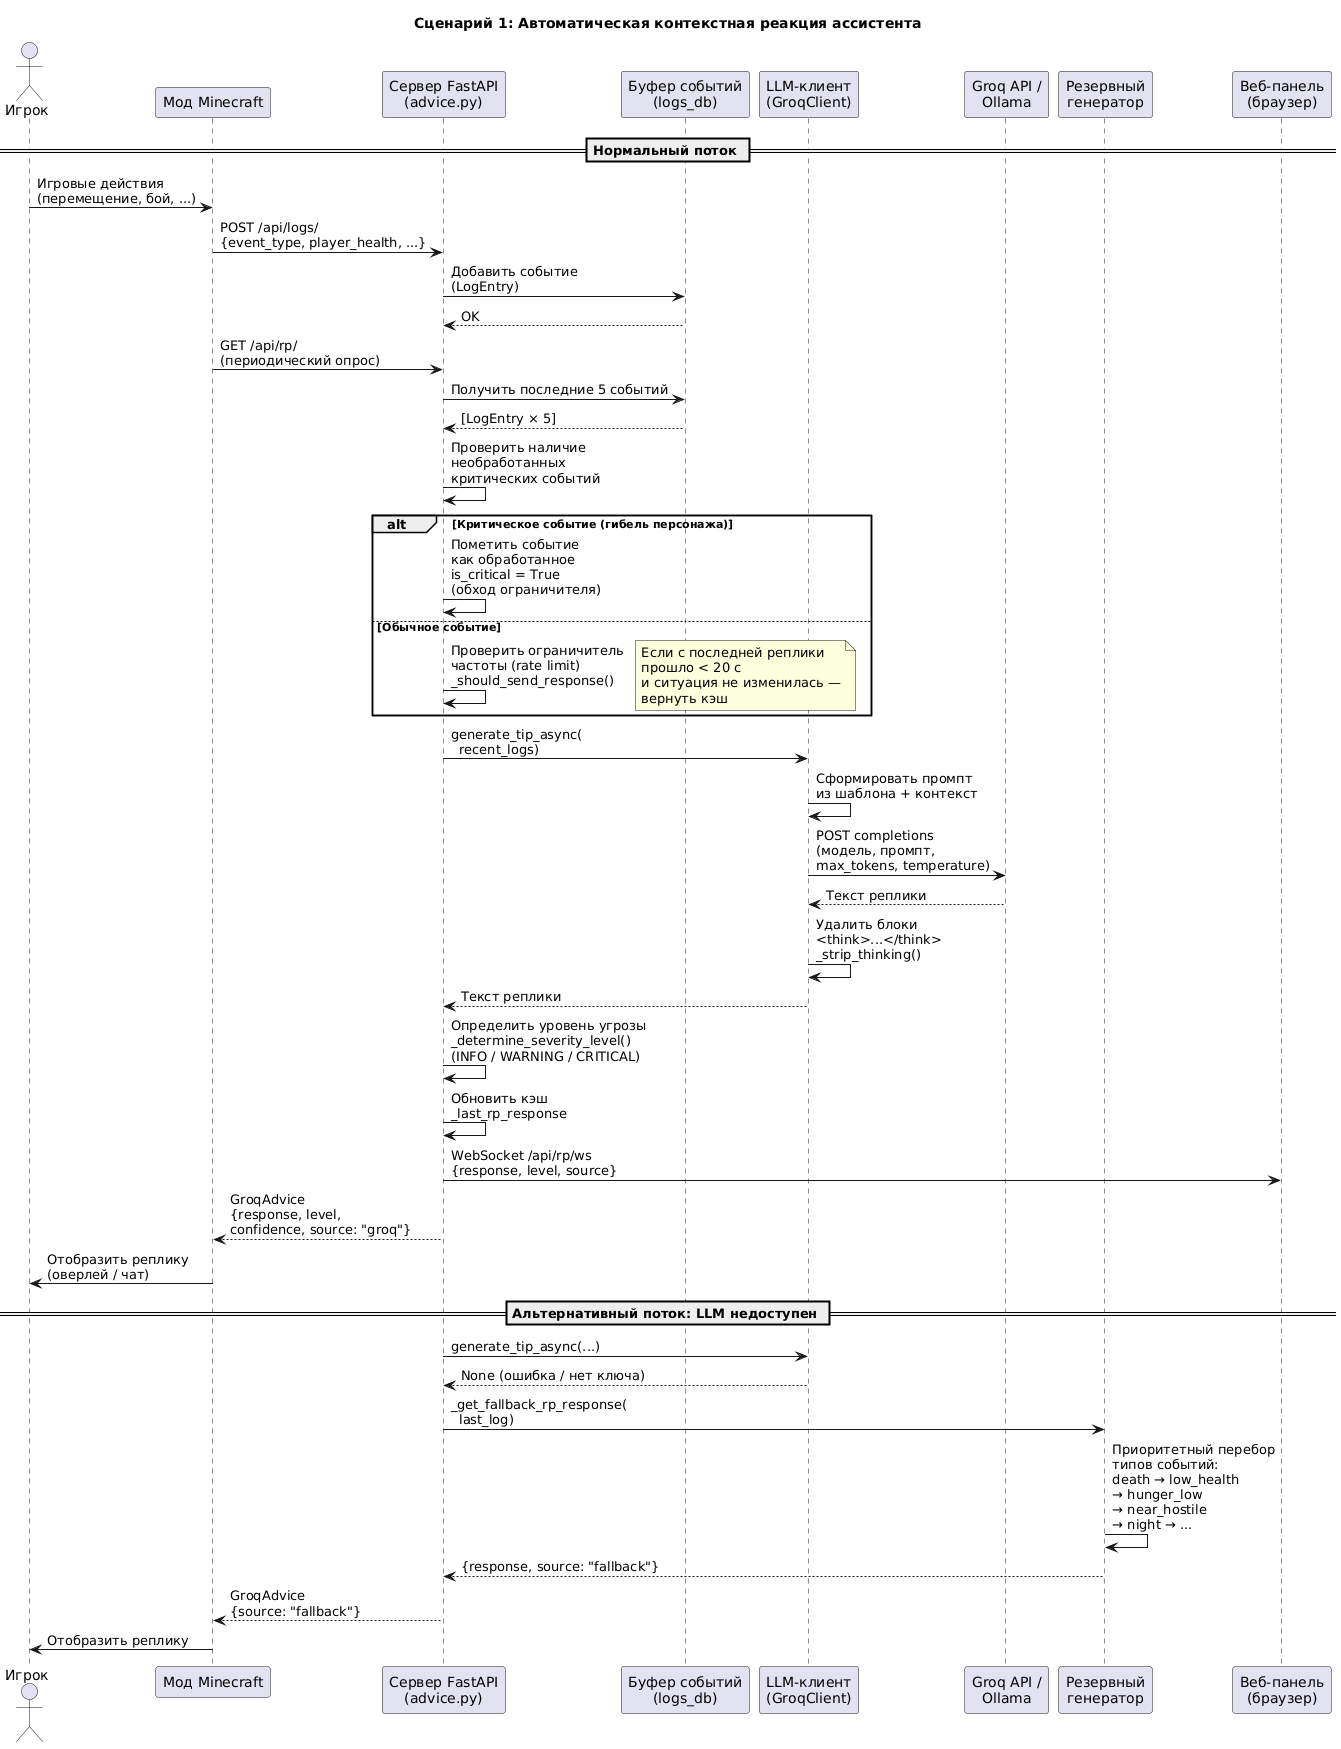
\includegraphics[scale=0.35]{picture/sequence1.png}
    \caption{Диаграмма последовательности для сценария 1}
    \label{fig:sequence1}
\end{figure}

\begin{figure}[H]
    \centering
    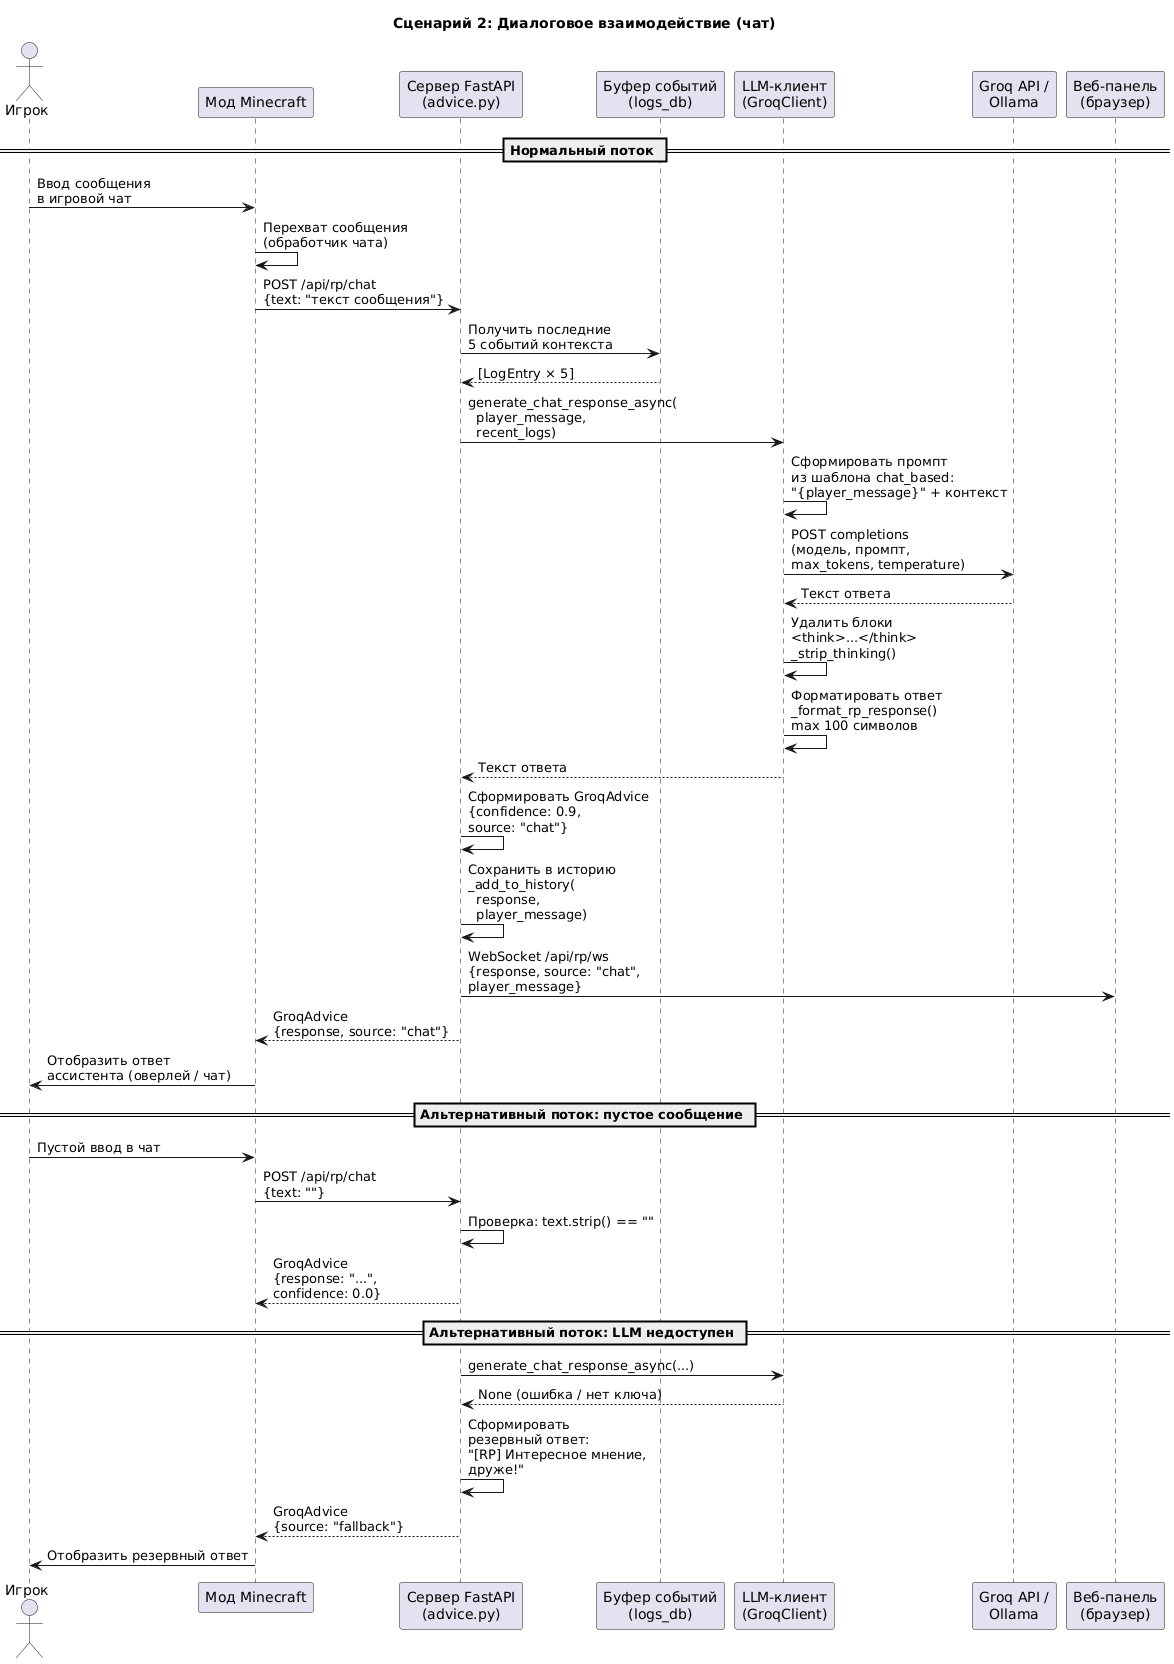
\includegraphics[scale=0.35]{picture/sequence2.png}
    \caption{Диаграмма последовательности для сценария 2}
    \label{fig:sequence2}
\end{figure}

\begin{figure}[H]
    \centering
    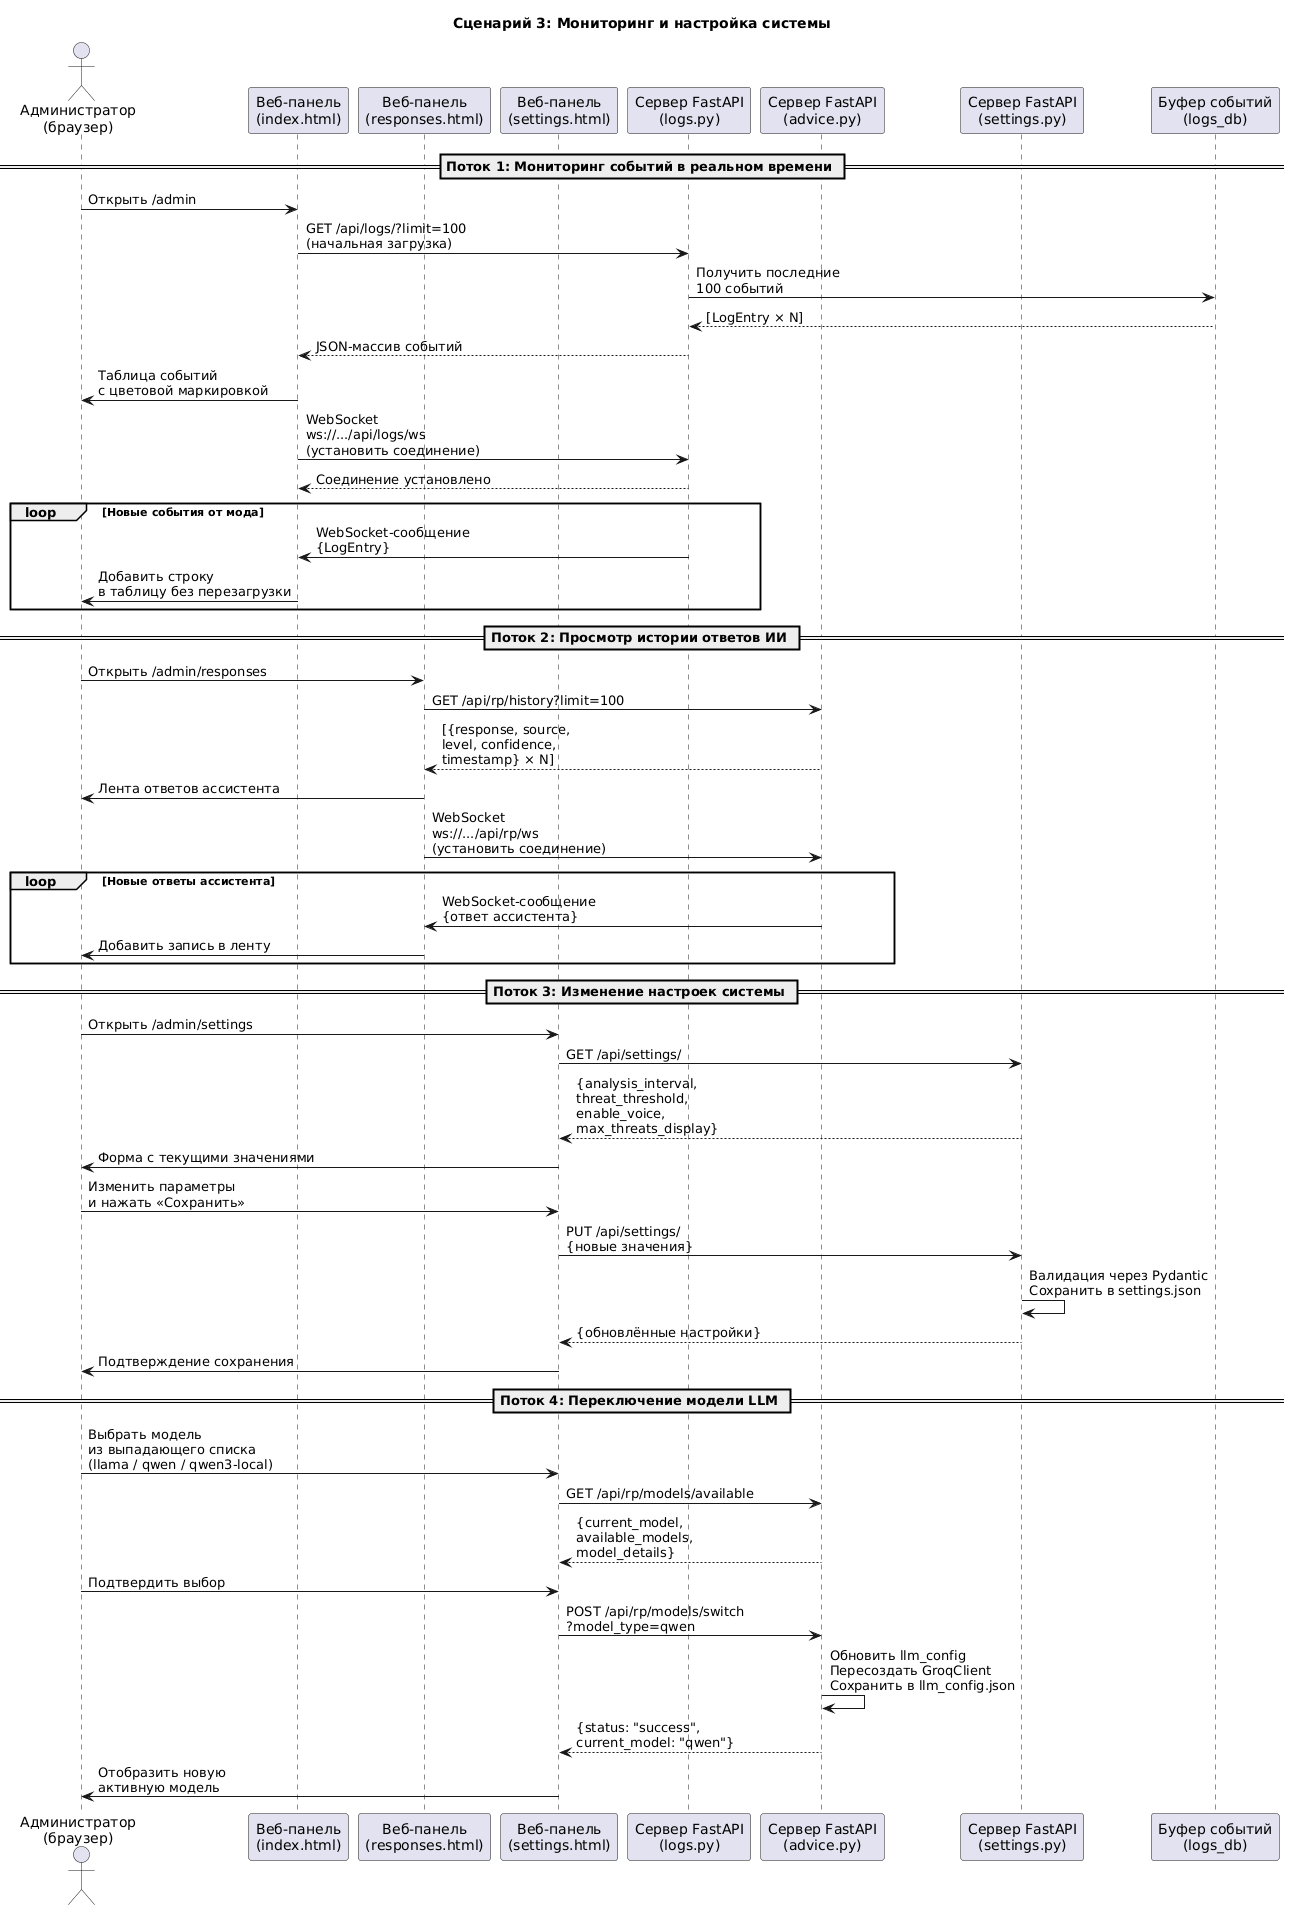
\includegraphics[scale=0.35]{picture/sequence3.png}
    \caption{Диаграмма последовательности для сценария 3}
    \label{fig:sequence3}
\end{figure}

\subsection{Проектирование пользовательского интерфейса}

\textbf{Информационная структура и навигация}

Административная веб-панель включает три самостоятельных страницы с навигацией через общий заголовок. Страница мониторинга событий предоставляет таблицу входящих данных от игрового клиента с указанием типа, уровня важности и временной метки каждого события. Страница истории ответов отображает ленту сгенерированных реплик ассистента с информацией об источнике ответа и уровне угрозы. Страница настроек позволяет изменять параметры работы системы и выбирать языковую модель.

\textbf{Макеты экранов и элементы управления}

На странице мониторинга строки таблицы окрашиваются в зависимости от уровня важности события, что позволяет быстро выделить критические ситуации. Обновление таблицы происходит без перезагрузки страницы по мере поступления новых данных.

На странице настроек сосредоточены поля для изменения числовых параметров системы: интервала анализа, порога угрозы и максимального числа отображаемых угроз. Отдельный элемент управления позволяет включить голосовой вывод реплик. Выпадающий список доступных языковых моделей с кнопкой применения обеспечивает переключение активного провайдера без перезапуска системы.

\subsection{Проектирование программного интерфейса}

\textbf{Спецификация операций и сообщений}

Серверный интерфейс включает три группы операций. Группа управления событиями обеспечивает приём данных от игрового клиента и предоставление журнала событий внешним потребителям. Группа управления реакциями ассистента позволяет запрашивать автоматически формируемую реплику по текущей игровой ситуации, а также отправлять сообщение игрока для получения ответа в режиме диалога; к этой же группе относятся операции просмотра доступных языковых моделей и переключения между ними. Группа управления настройками предоставляет возможность чтения и обновления рабочих параметров системы.

Для передачи данных в реальном времени предусмотрены два постоянных соединения: одно транслирует новые события по мере их поступления, второе — новые реплики ассистента. Оба канала используются административной панелью для отображения актуальной информации без перезагрузки страницы.

\textbf{Контракты и протоколы взаимодействия}

Все запросно-ответные операции выполняются по протоколу REST, данные передаются в формате JSON. Потоковые каналы реализованы на основе протокола WebSocket. Схемы данных строго типизированы: нарушение структуры входящего сообщения приводит к возврату ошибки с описанием несоответствия, что исключает некорректные данные в буфере событий.

Основные структуры данных включают: запись о событии с временной меткой, типом и уровнем важности, числовыми показателями состояния персонажа и сведениями об обнаруженных угрозах; набор настроек системы с параметрами интервала анализа и пороговых значений; структуру ответа ассистента с текстом реплики, уровнем угрозы, оценкой уверенности и указанием источника формирования ответа.

\subsection{Проектирование интеллектуальных механизмов интерфейса}

\textbf{Интеллектуальная поддержка пользователя}

Механизм формирования реплик работает в двух режимах с автоматическим выбором между ними. В основном режиме запрос к языковой модели составляется из шаблона, заданного в конфигурации, и описания текущей игровой ситуации на основе последних событий. Система поддерживает несколько профилей языковых моделей: облачные решения, доступные через внешний API, и локально развёртываемые модели, не требующие передачи данных во внешние сети. Выбор профиля производится через веб-панель без остановки сервера.

В резервном режиме, который активируется при недоступности языковой модели, ответ формируется детерминированной системой правил. Правила упорядочены по приоритету угрозы: наиболее критичные ситуации обрабатываются первыми, менее срочные — в порядке убывания опасности.

\textbf{Объяснимость и адаптация интерфейса}

Для предотвращения информационного перегруза реализован механизм ограничения частоты выдачи реплик. Повторная реплика не генерируется, пока не истечёт заданный минимальный интервал и пока игровая ситуация не изменится существенным образом. Критические события обходят это ограничение и всегда вызывают немедленную реакцию.

Каждый ответ ассистента сопровождается указанием источника его формирования — языковая модель или система правил — и уровнем угрозы, отражающим текущее состояние персонажа. Такая атрибуция позволяет администратору при анализе истории оценивать качество работы обоих режимов. Адаптация поведения системы обеспечивается настраиваемым порогом угрозы: при его превышении тональность и характер реплик меняются в соответствии с уровнем опасности.

\subsection{Вывод по разделу проектирования}

В ходе проектирования сформированы следующие ключевые архитектурные решения. Трёхуровневая клиент-серверная архитектура с чётким разделением ответственности обеспечивает независимость компонентов: замена языковой модели или резервной логики не затрагивает интерфейс взаимодействия с игровым клиентом. Двухуровневая схема деградации — основная генерация через языковую модель с автоматическим переключением на систему правил — обеспечивает надёжность ассистента при отказе внешних сервисов. Асинхронная обработка всех внешних запросов исключает блокировку сервера и поддерживает приемлемое время отклика. Конфигурируемые профили языковых моделей и сохраняемые настройки обеспечивают гибкость без изменения кода.

Предусмотрена возможность расширения: добавление новых типов игровых событий не требует изменения сервисного уровня, подключение новых языковых провайдеров осуществляется через конфигурационный файл, а интеграция синтеза речи выполняется включением соответствующего параметра без переработки программного интерфейса.
